\section{Introduction}
The \emph{camera pose}, known also as \emph{camera extrinsics}, can be expressed as a combination of two components:
\begin{enumerate}
    \item a tuple of three elements that identifies the absolute coordinates $x,y\text{ and }z$ in a reference space:
          \begin{equation}
              x_c=(x,y,z)\quad x,y,z \in \mathbb{R}
              \label{eq:absolute-position-definition}
          \end{equation}
    \item a quaternion of four elements that identifies the rotation of the camera:
          \begin{equation}
              q_c=(qw, qx, qy, qz)\quad qw,qx,qy,qz \in \mathbb{R}
              \label{eq:quaternion-as-rotation-definition}
          \end{equation}

\end{enumerate}
Consequentially, the pose is referred as $p_c=(x_c, q_c)$.

It is important to notice that this is not the only available representation for poses: other methods are based also on rotation matrices and Euler angles. It is worth specifying that even if Euler angles are the most straightforward and efficient in terms of memory consumption, they suffer from of the Gimbal lock problem. Also, although rotation matrices guarantee a good representation, they are more memory expensive (9 values) than quaternions (only 4 values): for this reason the latter form is preferred in this work.

Given an image $I_c$ captured by a camera $C$, an absolute pose estimator $E$ tries to predict the 3D pose orientation and location of $C$ in world coordinates, defined for some arbitrary reference system in the 3D model. Formally speaking, the \emph{absolute pose estimation (APE)} problem can be defined as the problem of estimating a function $E$ taking as input an image $I_c$ captured by a camera $C$ and as output its respective pose:
\begin{equation}
    E(I_c) = (x_c, q_c)
    \label{eq:absolute-pose-estimation-task}
\end{equation}

\begin{figure}[h]
    \begin{center}
        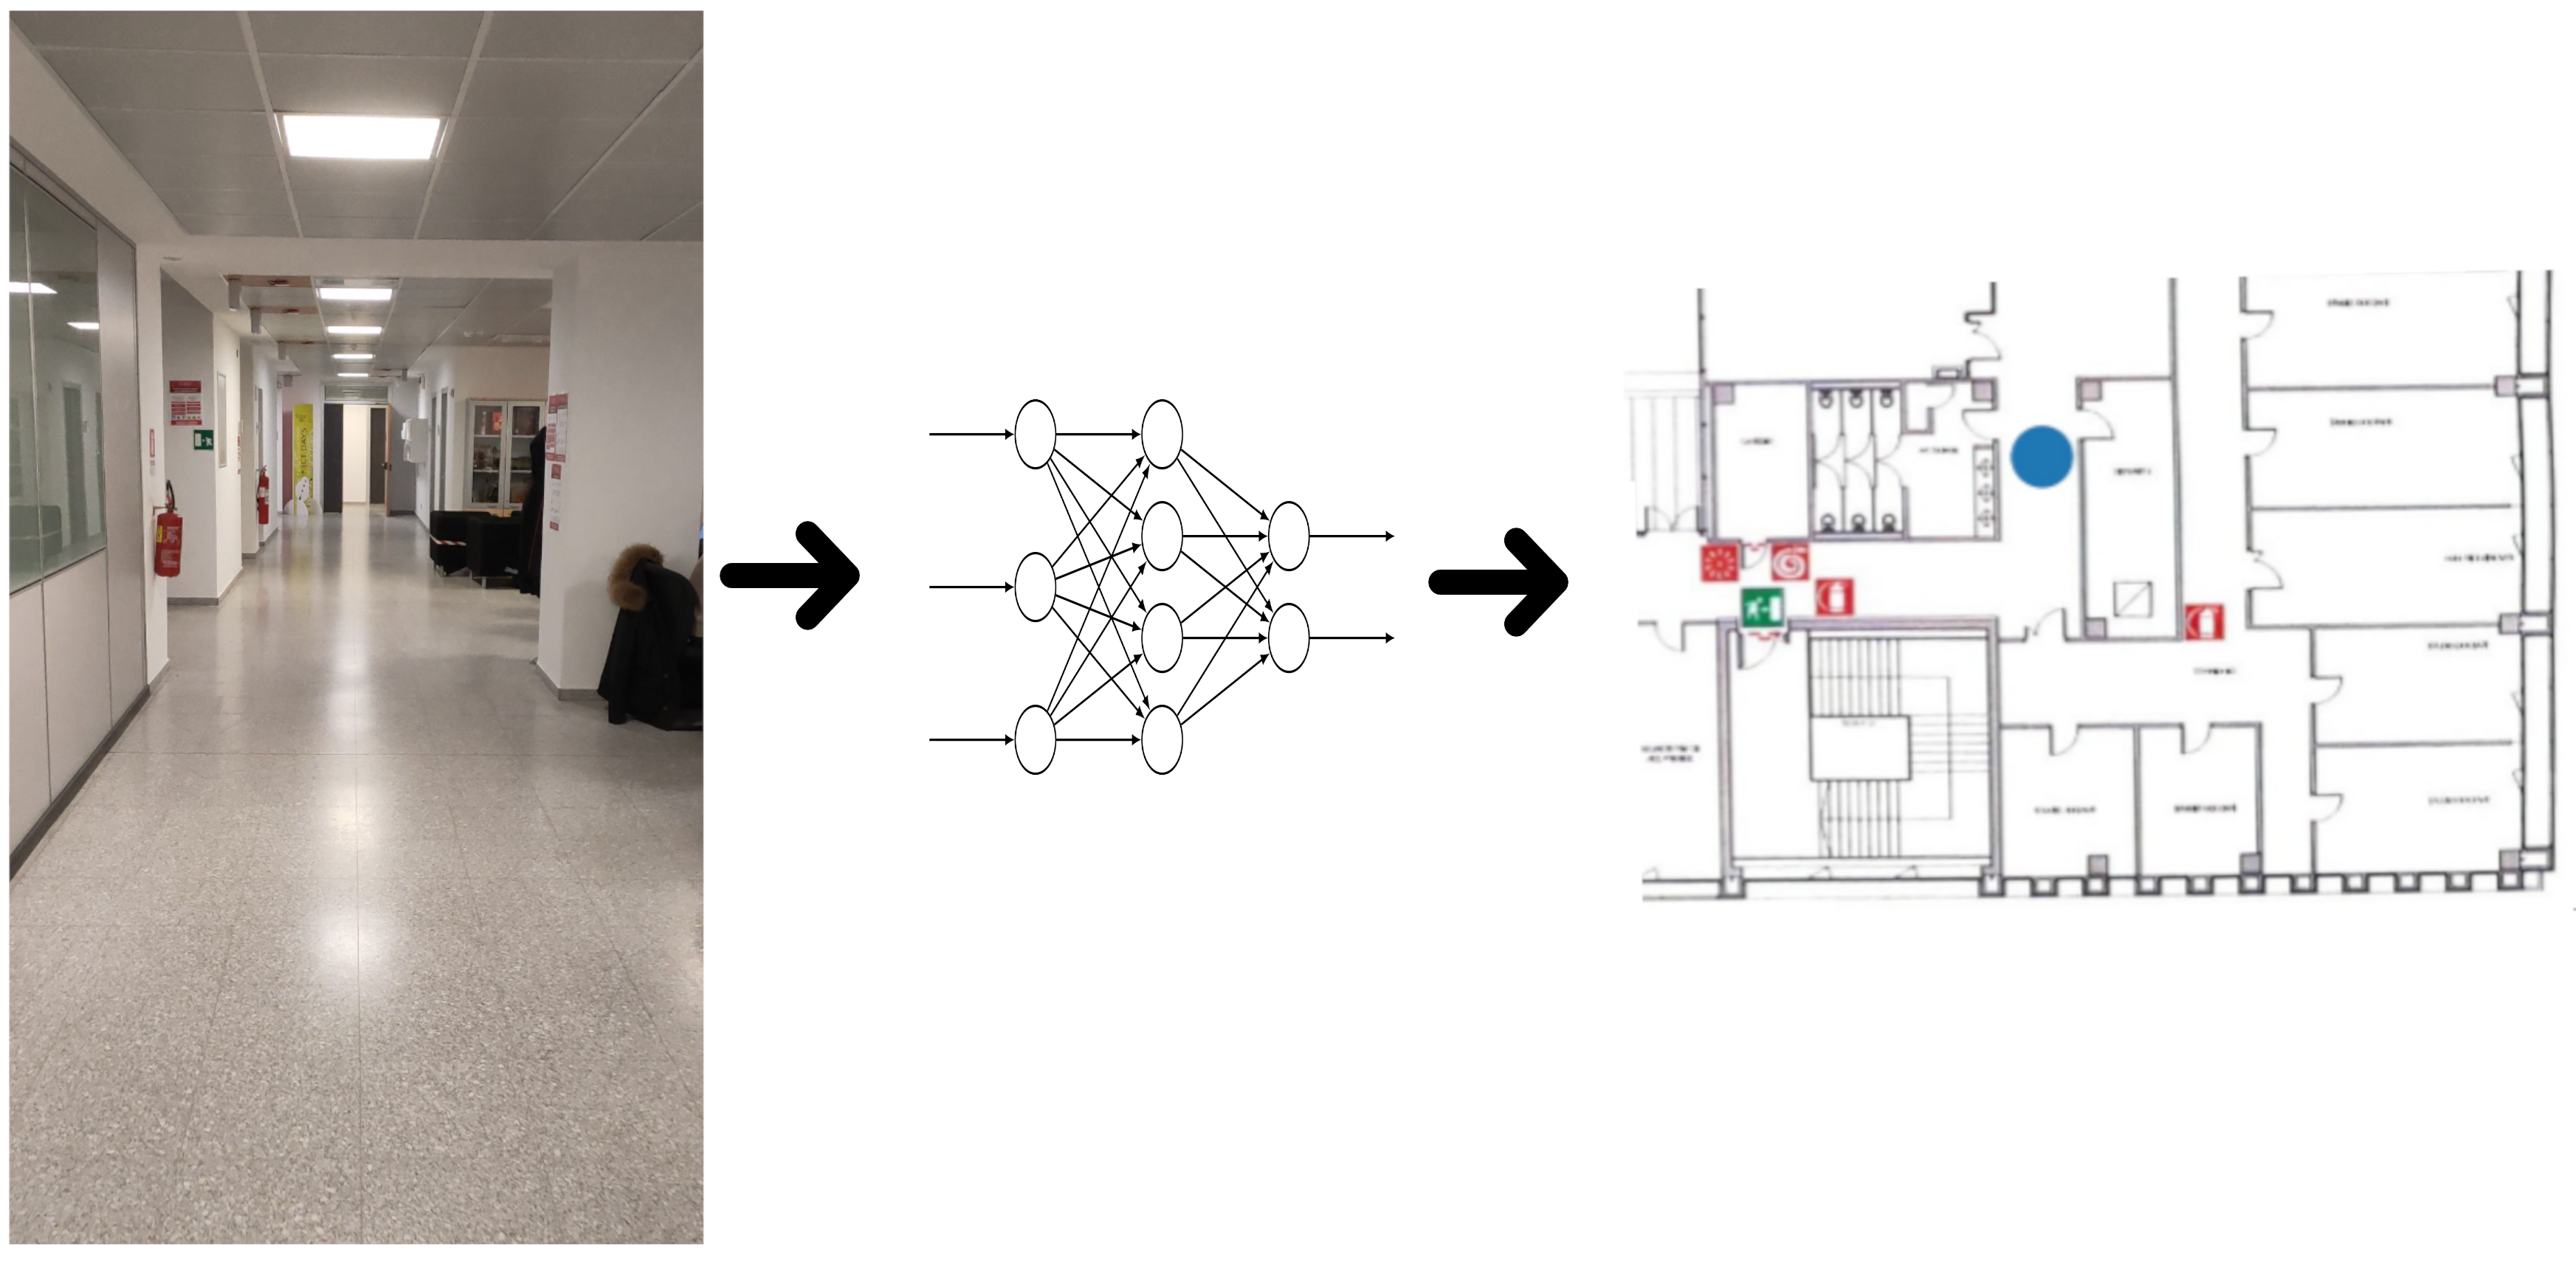
\includegraphics[width=0.48\textwidth]{./imgs/introduction_example.png}
    \end{center}
    \caption{How an APE deep learning model works.}
    \label{fig:introduction-example}
\end{figure}

Apart from APE, another popular task is also \emph{relative pose estimation (RPE)}. In this kind of approach the estimator takes two images $I_c^1$ and $I_c^2$ captured by $C$ and aims to predict the relative pose between them. In this case, the formulation of the function $E$ described in \cref{eq:absolute-pose-estimation-task} is a little different, since it receives as input two images:
\begin{equation}
    E(I_c^1, I_c^2) = (x_c^{rel}, q_c^{rel})
    \label{eq:relative-pose-estimation-task}
\end{equation}
where $(x_c^{rel}, q_c^{rel})$ is defined as the absolute pose with \emph{coordinates reference system} in $I_c^1$ or, in an equivalent way, as the translation vector from $I_c^1$ to $I_c^2$.

With this work, we show how it is possible to build a deep learning model which is able to learn the function $E$ using a data-driven approach.

In both scenarios, the estimator can be viewed as a model which describes an environment that can be questioned about the pose of an element within it.
